\documentclass[preprint,12pt]{elsarticle}

    \usepackage[sc]{mathpazo} % Use the Palatino font
    \usepackage[T1]{fontenc} % Use 8-bit encoding that has 256 glyphs
    \usepackage{microtype} % Slightly tweak font spacing for aesthetics
    \usepackage[english]{babel} % Language hyphenation and typographical rules
    \usepackage{booktabs} % Horizontal rules in tables
    \usepackage{enumitem} % Customized lists
    \usepackage[table,xcdraw]{xcolor}
    \usepackage[utf8]{inputenc} % Required for inputting international characters
    \usepackage{parskip}
    \usepackage{graphicx}
    \usepackage{hyperref}
    \usepackage{pdfpages}
    \usepackage{amsmath}
    \usepackage{esvect}
    \usepackage{listings}
    \usepackage{color}
    \usepackage{spverbatim}
    \usepackage{subcaption}
    \usepackage[title]{appendix}
    \hypersetup{
        colorlinks=true,
        linkcolor=blue,
        filecolor=magenta,      
        urlcolor=cyan,
    }
    \definecolor{dkgreen}{rgb}{0,0.6,0}
    \definecolor{gray}{rgb}{0.5,0.5,0.5}
    \definecolor{mauve}{rgb}{0.58,0,0.82}
    \definecolor{lightgray}{rgb}{0.83, 0.83, 0.83}
    \definecolor{timberwolf}{rgb}{0.86, 0.84, 0.82}
    \definecolor{whitesmoke}{rgb}{0.96, 0.96, 0.96}
    
    \lstset{frame=tb,
    language=python,
    aboveskip=3mm,
    belowskip=3mm,
    showstringspaces=false,
    columns=flexible,
    basicstyle={\small\ttfamily},
    numbers=none,
    numberstyle=\tiny\color{gray},
    keywordstyle=\color{blue},
    commentstyle=\color{dkgreen},
    stringstyle=\color{mauve},
    breaklines=true,
    breakatwhitespace=true,
    tabsize=3,
    backgroundcolor = \color{whitesmoke}
    }

    \begin{document}
    \title{\LARGE \bf
        STAT 391 Homework 2
        }
        
        \author{ \parbox{3 in}{\centering Chongyi Xu \\
                 University of Washington\\
                 STAT 391 Spring 2018\\
                 {\tt\small chongyix@uw.edu}}
        }
    \maketitle

    \section{Problem 1 - CDF's and densities}
    Let
    \begin{equation*}
        F(x) = 
        \begin{cases}
            0,  &x\leq 0\\
            x^2, &0<x\leq 1\\
            1,  &1<x
        \end{cases}
    \end{equation*}
    and
    \begin{equation*}
        G(x) =
        \begin{cases}
            0,          &x\leq 0\\
            2x^2,       &0<x\leq 0.5\\
            1-2(1-x)^2, &0.5<x\leq 1\\
            1,          &1<x
        \end{cases}
    \end{equation*}
    be two cumulative distribution functions.
    \begin{enumerate}
        \item Plot F, G
        \begin{lstlisting}
import numpy as np
import matplotlib.pyplot as plt

x = np.arange(0,1,step=0.01)
F = [xx**2 for xx in x]
G = np.empty([len(x), 1])
for xx in x:
    if xx <= 0.5:
        G[x==xx] = 2 * xx**2
    elif xx <= 1:
        G[x==xx] = 1 - 2 * (1 - xx)**2
plt.figure()
plt.plot(x, F, 'r--', label='F(x)')
plt.plot(x, G, 'g^', label='G(x)')
plt.xlabel('x')
plt.title('F(x) and G(x)')
plt.legend()
plt.show()
        \end{lstlisting}
        \begin{figure}[htbp!]
            \center
            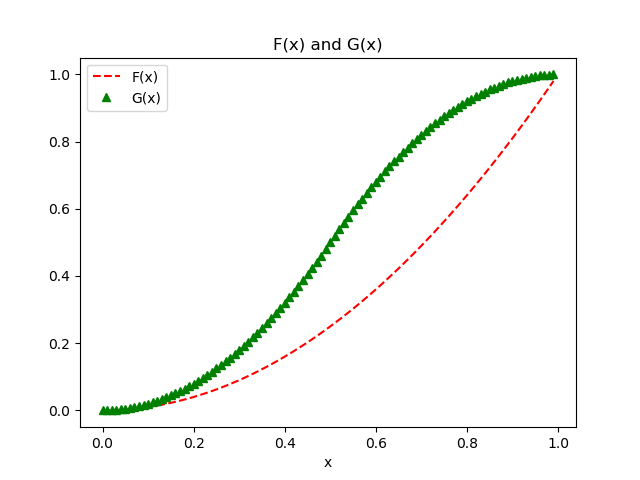
\includegraphics[width = \textwidth]{1.png}
            \caption{CDF: F, G}
            \label{fig:1}
        \end{figure}
    
    \item Compute their corresponding desensitize f, g. Plot them on a 
    graph.
    \begin{align*}
        f_X(x) &= \frac{d}{dx}F_X(x)    &&=
        \begin{cases}
            0,  &x\leq 0\\
            2x, &0<x\leq 1\\
            0,  &1<x
        \end{cases} \\
        g_X(x)  &= \frac{d}{dx}G_X{x}   &&=
        \begin{cases}
            0,          &x\leq 0\\
            4x,         &0<x\leq 0.5\\
            4(1-x),     &0.5<x\leq 1\\
            0,          &1<x
        \end{cases}
    \end{align*}
    \begin{lstlisting}
f = [2*xx for xx in x]
g = np.empty([len(x), 1])
for xx in x:
    if xx <= 0.5:
        g[x==xx] = 4 * xx
    elif xx <= 1:
        g[x==xx] = 4 * (1-xx)
plt.figure()
plt.plot(x, f, 'r--', label='f(x)')
plt.plot(x, g, 'g^', label='g(x)')
plt.xlabel('x')
plt.title('Density f(x) and g(x)')
plt.legend()
plt.show()    
    \end{lstlisting}
    \begin{figure}[htbp!]
        \center
        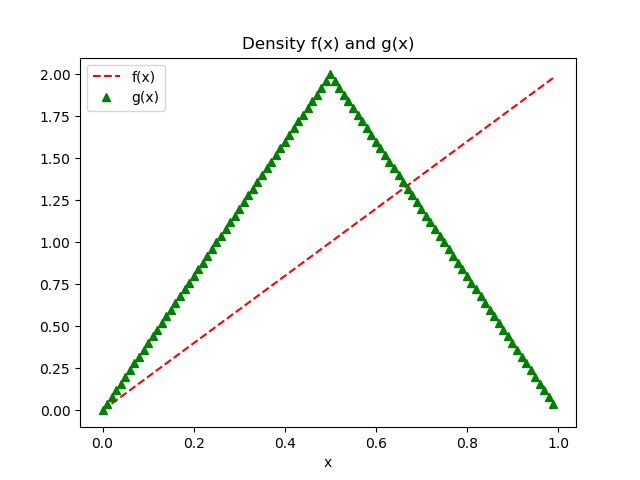
\includegraphics[width = \textwidth]{2.png}
        \caption{pdf: f, g}
        \label{fig:2}
    \end{figure}

    \item Denote by $P_F$ and $P_G$ the probability distribution defined
    by $F,G$. Find $a,a^{'}$ such that $P_F(0,a)=P_F(a,1)$ and 
    $P_G(0,a^{'})=P_G(a^{'},1)$.\\

    Since $P(\alpha,\beta) = P_X(x\leq \beta) - P_X(x\leq \alpha)$. Therefore,
    \begin{align*}
        P(0, a)     &= P(a, 1) \\
        F_X(a) - F_X(0)     &= F_X(1) - F_X(a) \\
        \Rightarrow 2F_X(a) &= F(0) + F(1) = 1 \\
                    F_X(a)  &= \frac{1}{2} \\
                        a   &= \frac{\sqrt{2}}{2} \\
        G_X(a^{'}) - G_X(0)     &= G_X(1) - G_X(a^{'}) \\
        \Rightarrow 2G_X(a^{'}) &= 1 \\
                    G_X(a^{'})  &= \frac{1}{2}\\
                    a^{'}       &= \frac{1}{2} \\
    \end{align*}
    \\
    \begin{figure}[htbp!]
        \center
        \begin{subfigure}{0.8\textwidth}
            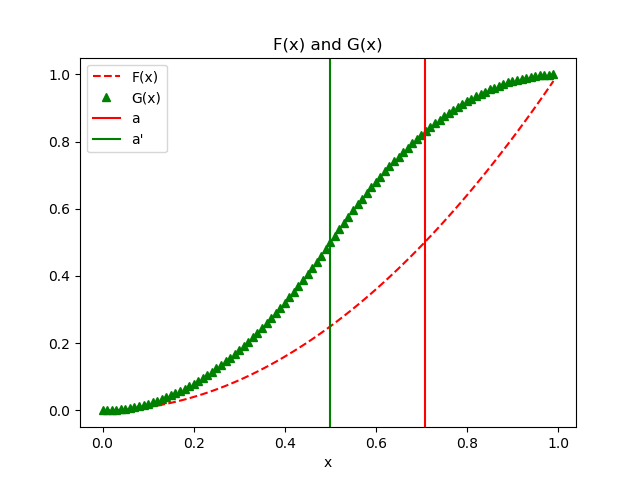
\includegraphics[width = \textwidth]{3.png}
            \caption{CDF with $a$ and $a^{'}$}
            \label{fig:3-1}
        \end{subfigure}
        \begin{subfigure}{0.8\textwidth}
            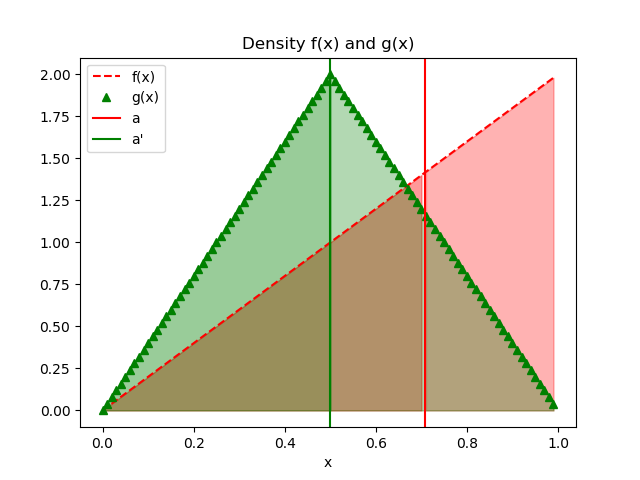
\includegraphics[width = \textwidth]{4.png}
            \caption{PDF with $a$ and $a^{'}$}
            \label{fig:3-2}
        \end{subfigure}
        \caption{Plot with $a$ and $a^{'}$}
        \label{fig:3}
    \end{figure}
    From the plot Figure \ref{fig:3-2}, we could see that the left part and 
    right part has about same area under the curve on the sides of $a$ and 
    $a^{'}$, which is a way to verify my $a$ and $a^{'}$ are correct.

    \item Find the probabilities of the following intervals $[0,0.25]$,
    $[1,1.75]$ under $P_F,P_G$.
    \begin{align*}
        P_F(x\in[0,0.25])   &= F_X(x=0.25) - F_X(x=0) \\
                            &= \frac{1}{16} \\
        P_G(x\in[0,0.25])   &= G_X(x=0.25) - G_X(x=0) \\
                            &= \frac{2}{16} = \frac{1}{8} \\
        P_F(x\in[1,1.75])   &= 1-1=0 = P_G(x\in[1,1.75])
    \end{align*}

    \item Find the shortest interval $[a_F, b_F]$ that has probability
    0.1 under F. Find $[a_G, b_G]$ under G.
    \begin{lstlisting}
[af, ag, bf, bg] = [-float('inf'), -float('inf'), float('inf'), float('inf')]
x = np.arange(0,1,step=0.001)
F = np.array([xx**2 for xx in x])
G = np.empty([len(x), 1])
for xx in x:
    if xx <= 0.5:
        G[x==xx] = 2 * xx**2
    elif xx <= 1:
        G[x==xx] = 1 - 2 * (1 - xx)**2
G = G[:,0]
for i in range(len(x)):
    xa = x[i]
    for j in range(i+1, len(x)):
        xb = x[j]
        if (F[x==xb] - F[x==xa] == 0.1) and\
             (xb - xa < bf - af):
            [af, bf] = [xa, xb]
        if (G[x==xb] - G[x==xa] == 0.1) and\
            (xb - xa < bg - ag):
            [ag, bg] = [xa, xb]

print('[a_f, b_f]='+str([af,bf]))
print('[a_g, b_g]='+str([ag,bg]))
    \end{lstlisting}
    So within a step of $0.001$, I found my shortest interval to be
    \begin{align*}
        [a_F, b_F]  &= [0.075, 0.325] \\
        [a_G, b_G]  &= [0.025, 0.225]
    \end{align*}
    \begin{lstlisting}
plt.figure()
plt.plot(x, f, 'r--', label='f(x)')
plt.plot(x, g, 'g^', label='g(x)')
plt.axvline(x=af, color='r', linestyle='solid')
plt.axvline(x=bf, color='r', linestyle='solid')
plt.axvline(x=ag,  color='g', linestyle='solid')
plt.axvline(x=bg,  color='g', linestyle='solid')
plt.fill_between(x, 0, f, where=np.logical_and(x>=af, x<=bf), color='red', alpha=0.3)
plt.fill_between(x, 0, g, where=np.logical_and(x>=ag, x<=bg), color='green', alpha=0.3)
plt.xlabel('x')
plt.title('Density f(x) and g(x)')
plt.legend()
plt.show()
    \end{lstlisting}
    \begin{figure}[htbp!]
        \center
        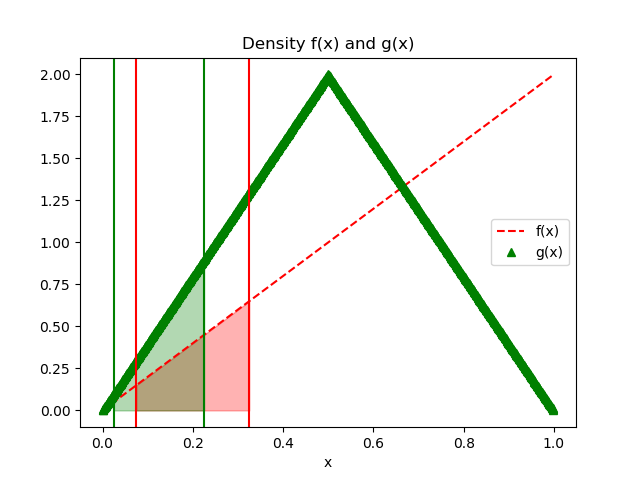
\includegraphics[width=0.8\textwidth]{5.png}
        \caption{Intervals of $a_F,b_F,a_G,b_G$}
        \label{fig:5}
    \end{figure} 
    Showing the intervals on the graphs of f, g on Figure \ref{fig:5}

    \item Calculate the means of $f,g$, denoted by $E_f[X],E_g[X]$.
    \begin{lstlisting}
print('E_f[x]=' + str(np.mean(f)))
print('E_g[x]=' + str(np.mean(g)))
    \end{lstlisting}
    \begin{spverbatim}
    E_f[x]=0.999
    E_g[x]=1.0
    \end{spverbatim}
    \end{enumerate}

    \section{Problem 2}
    \begin{enumerate}
        \item Denote by $p_n$ the probability of the interval $[n-1, n)$ 
        under the exponential distribution. What is the expression of 
        $p_n$ as a function of $\gamma$ and $n$? What is this expression 
        if $\gamma=ln2$?
        \begin{align*}
            p_n     &= Pr(x\in [n-1, n)) \\
                    &= Pr(x<n) - Pr(x\leq n-1) \\
                    &= 1 - e^{-\gamma n} - (1 - e^{-\gamma (n-1)}) \\
                    &= e^{-\gamma (n-1)} - e^{-\gamma n} \\
                    &= e^{-\gamma}(e^{n\gamma} - e^n)
                    &= e^{-\gamma n}(e^{\gamma} - 1)
        \end{align*}
        If $\gamma=ln2$, plugging in,
        \begin{equation*}
            p_n = e^{-ln(2)}(e^{n\cdot ln(2) - e^n}) = \frac{1}{2}(2e^n - e^n)
        \end{equation*}

        \item What is the expression of $\frac{p_n}{p_{n+1}}$ as a function
        of $\gamma$ and $n$? What is the expression if $\gamma=ln2$?
        \begin{align*}
            p_{n+1} &= e^{-\gamma}(e^{(n+1)\gamma} - e^{n+1}) \\
                    &= e^{-\gamma n}(1 - e^{-\gamma}) \\
            \frac{p_n}{p_{n+1}}     &= \frac{e^{\gamma} - 1}{1 - e^{-\gamma}} 
        \end{align*}
        If $\gamma=ln2$, plugging in,
        \begin{equation*}
            \frac{p_n}{p_{n+1}} = \frac{2 - 1}{1 - 1/2} = 2 
        \end{equation*}

        \item Plot on the same graph the densities $f_{\gamma}(x)$ for 
        $\gamma=ln2,ln3,ln4$.
        \begin{lstlisting}
import math
import numpy as np
import matplotlib.pyplot as plt

gamma = [math.log(2), math.log(3), math.log(4)]
x = np.arange(0, 10, step=0.01)
fx = np.empty([len(gamma), len(x)])
for k in range(len(gamma)):
    fx[k,] = [gamma[k] * math.exp(-gamma[k] * xx) for xx in x]

plt.figure()
plt.plot(x, fx[0,], 'r--', label='gamma=ln(2)')
plt.plot(x, fx[1,], 'g--', label='gamma=ln(3)')
plt.plot(x, fx[2,], 'b--', label='gamma=ln(4)')
plt.xlabel('x')
plt.title('Density f(x) for different gammas')
plt.legend()
plt.show()
        \end{lstlisting}
        \begin{figure}[htbp!]
            \center
            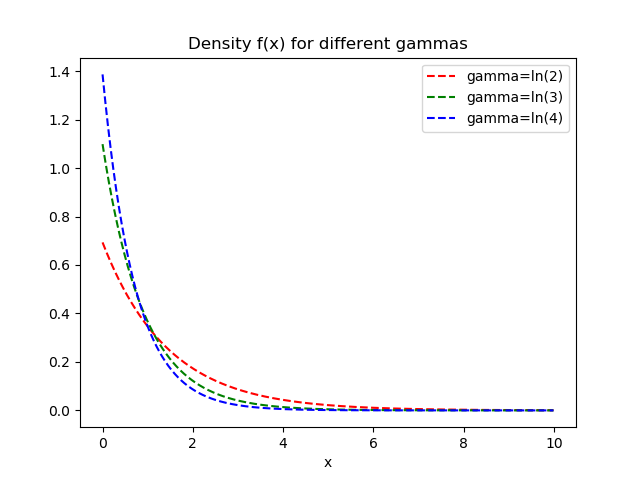
\includegraphics[width=0.8\textwidth]{6.png}
            \caption{Densities of $f_{\gamma}(x)$ for $\gamma=$ln2,ln3,ln4}
            \label{fig:6}
        \end{figure}
        Figure \ref{fig:6} shows the density curves.

        \item Let $g(x) = \frac{1}{Z} e^{-\gamma(x+3)}$, Evaluate the
        normalization constant $Z$ as a function of $\gamma$. Evaluate
        the expression of the CDF $G$ of this distribution.\\

        Using the fact that the integral of a density function over the 
        interval $(-\infty, +\infty)$ is $1$.
        \begin{align*}
            \int_{-3}^{\infty} \frac{1}{Z} e^{-\gamma(x+3)}dx &= 1\\
            \int_{-3}^{\infty} e^{-\gamma x - 3\gamma}dx &= Z\\
            -\frac{1}{\gamma}e^{-\gamma x} \Big|_{-3}^{\infty} &= Ze^{3\gamma} \\
            0 + \frac{1}{\gamma}e^{3\gamma} &= Ze^{3\gamma} \\
            \Rightarrow Z &= \frac{1}{\gamma}
        \end{align*}

        And therefore, we have our CDF $G_X(x)$ to be 
        \begin{align*}
            G_X(x) &= \int_{-3}^{x} \gamma e^{-\gamma(x+3)}dx\\
                    &= \gamma e^{-3\gamma}\int_{-3}^{x} e^{-\gamma x}dx\\
                    &= \gamma e^{-3\gamma}\frac{1}{-\gamma}e^{-\gamma x} \Big|_{-3}^{x}\\
                    &= -e^{-3\gamma}(e^{-\gamma x} - e^{3\gamma}) \\
                    &= 1 - e^{-\gamma(x+3)}
        \end{align*}
    \end{enumerate}

    \section{Problem 3}
    \begin{enumerate}
        \item Make a sketch of densities $f_X, f_Y$.
        \begin{lstlisting}
import numpy as np
import matplotlib.pyplot as plt

x = np.arange(0,3,step=0.01)
fx= np.zeros([len(x), 1])
fy= np.zeros([len(x), 1])
for xx in x:
    if xx >= 0.75 and xx <= 1.5:
        fy[x==xx] = 1/(1.5-0.75)
    if xx >=1 and xx<= 3:
        fx[x==xx] = 1/(3-1)
fx = fx[:,0]
fy = fy[:,0]
plt.figure()
plt.plot(x, fx, 'r-', label='f_X')
plt.plot(x, fy, 'b-', label='f_Y')
plt.xlabel('x')
plt.title('Densities of X and Y')
plt.legend()
plt.show()
        \end{lstlisting}
        \begin{figure}[htbp!]
            \center
            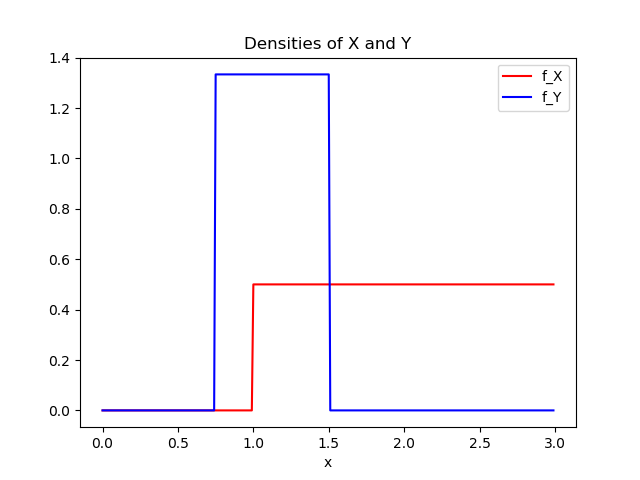
\includegraphics[width=0.8\textwidth]{7.png}
            \caption{Densities of $f_X$ and $f_Y$}
            \label{fig:7}
        \end{figure}
        Figure \ref{fig:7} shows the densities of rabbit's and fox's
        jump lengths.

        \item What are the CDF's of $x$ and $y$?
        \begin{align*}
            F_X(x)  &= \frac{x-1}{3-1} &&= \frac{x-1}{2},x\in [1,3]\\
            F_Y(y)  &= \frac{y-0.75}{1.5-0.75} &&= \frac{4y - 3}{3}, y\in [0.75, 1.5]
        \end{align*}
        \begin{lstlisting}
Fx= np.zeros([len(x), 1])
Fy= np.zeros([len(x), 1])
for xx in x:
    if xx >= 0.75 and xx <= 1.5:
        Fy[x==xx] = (4*xx-3)/3
    if xx >=1 and xx<= 3:
        Fx[x==xx] = (xx-1)/2
Fx = Fx[:,0]
Fy = Fy[:,0]
plt.figure()
plt.plot(x, Fx, 'r-', label='F_X')
plt.plot(x, Fy, 'b-', label='F_Y')
plt.xlabel('x')
plt.title('CDF of X and Y')
plt.legend()
plt.show()
        \end{lstlisting}
        \begin{figure}[htbp!]
            \center
            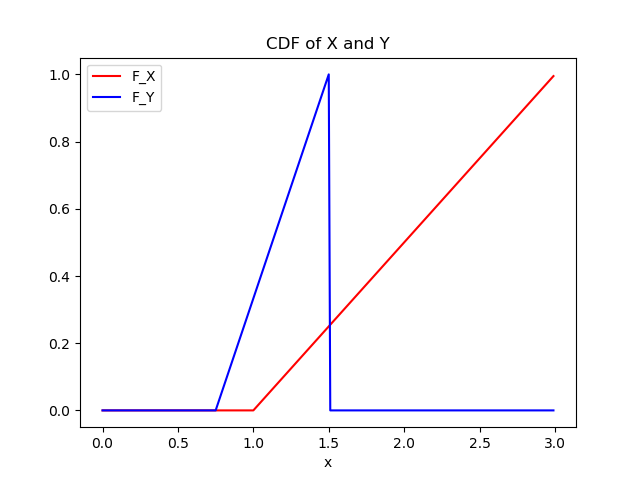
\includegraphics[width=0.8\textwidth]{8.png}
            \caption{$F_X$ and $F_Y$}
            \label{fig:8}
        \end{figure}
        Figure \ref{fig:8} shows the CDF of rabbit's and fox's
        jump lengths.

        \item What is the probability that a rabbit junps more than 2.5ft?
        What is the probability that a fox jumps less than 1ft?
        \begin{align*}
            Pr_X(x\geq 2.5) &= 1 - Pr_X(x\leq 2.5)\\
                            &= 1 - F_X(x=2.5)\\
                            &= 1 - \frac{2.5-1}{2} \\
                            &= 0.25
            Pr_Y(y\leq 1)   &= F_Y(y=1)\\
                            &= \frac{4*1-3}{3}\\
                            &\approx 0.33
        \end{align*}

        \item A fox is $d=1$ft away from an unsuspecting rabbit. What is the
        probability that the fox will catch the rabbit, if the fox jumps once
        directly towards the rabbit and the rabbit is too surprised to move?
        To catch a rabbit, this fox must land within 0.2 ft of the rabbit.
        \begin{align*}
            Pr_Y(y\geq (d-0.2)) &= 1 - Pr_Y(y\leq 0.8) \\
                                &= 1 - F_Y(y=0.8) \\
                                &= 1 - \frac{4*0.8-3}{3} \\
                                &\approx 0.93
        \end{align*}
        So the fox is has a probability of approximately 0.93 to catch the 
        rabbit with a $d=1$ ft away.

        \item The same question, assume $d=1.4ft$.
        \begin{align*}
            Pr_Y(y\geq (d-0.2)) &= 1 - Pr_Y(y\leq 1.2) \\
                                &= 1 - F_Y(y=1.2) \\
                                &= 1 - \frac{4*1.2-3}{3} \\
                                &= 0.4
        \end{align*}
        So the fox is has a probability of approximately 0.4 to catch the 
        rabbit with a $d=1.4$ ft away.

        \item The fox is now only 0.5 ft from the rabbit, but the rabbit also 
        takes a jump away from the fox. What is the probability that the fox 
        will catch the rabbit, assuming that the fox jumped $y = 1$ ft?\\

        Since we are look for the probability that the fox will catch the rabbit,
        and we know that the fox jumped $y=1$ ft. So, we need to find the
        probability that the rabbit is not able to flee from the fox. In the 
        other word, the rabbit has jumped less than $y+0.2-0.5=y-0.3$ ft.
        \begin{align*}
            Pr_X(x\leq (y-0.3)) &= Pr_X(x\leq 0.7) \\
                                &= 0
        \end{align*}
        So the fox will not be able to catch the rabbit under this condition.

        \item Make a plot of the probability that the fox catches the rabbit
        under the conditions in \textbf{f.}, as a function of $y$.
        \begin{figure}[htbp!]
            \center
            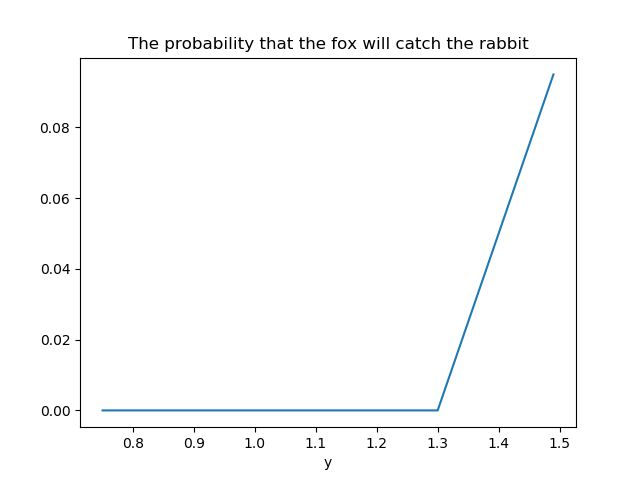
\includegraphics[width=0.8\textwidth]{9.png}
            \caption{The probability that the fox catches the rabbit as a function of $y$}
            \label{fig:9}
        \end{figure}
        Figure \ref{fig:9} shows the plot of probability that the fox can catch
        the rabbit under the given condition with the chaning $y$.
        \end{enumerate}

    \section{Problem 4- Rayleigh Distribution}
    \begin{enumerate}
        \item Write the formula of likelihood of $a$, $L(a)$.
        \begin{equation*}
            L(a) = \prod_{i=1}^n f(r_i|a) = \prod_{i=1}^n \frac{r_i}{a^2}e^{-\frac{r_i^2}{2a^2}}
        \end{equation*}

        \item Take the logarithm of $L(a)$ to obtain the log-likelihood 
        $l(a) = log L(a)$. Then compute the derivative
        \begin{align*}
            log L(a)    &= log \prod_{i=1}^n \frac{r_i}{a^2}e^{-\frac{r_i^2}{2a^2}}\\
                        &= \sum_{i=1}^n log(\frac{r_i}{a^2}e^{-frac{r_i^2}{2a^2}})\\
                        &= \sum_{i} [log(r_i) - 2log(a) - \frac{r_i^2}{2a^2}]\\
                        &= \sum_{i} [log(r_i) - \frac{r_i^2}{2a^2}] - 2nlog(a)
        \end{align*}
        Then, the derivative $\partial l/\partial a$ will be
        \begin{equation*}
            \frac{\partial l}{\partial a}  = \sum_{i=1}^n \frac{r_i^2}{a^3} - \frac{2n}{a}
        \end{equation*}

        \item Now solve the equation $\frac{\partial l}{\partial a}=0$ to obtain
        a formula for $a^{\text{M L}}$ as a function of the data.
        \begin{align*}
            \frac{\partial l}{\partial a}=0 &= \sum_{i=1}^n \frac{r_i^2}{a^3} - \frac{2n}{a}\\
                &= \sum_{i} \frac{r_i^2}{a^2} - 2n\\
                \frac{1}{a^2}   &= \frac{2n}{\sum r_i}\\
                a   &= \sqrt{\frac{\sum_{i} r_i}{2n}}
        \end{align*}

        \item Does this problem has sufficient statistics? What are they?\\

        In this problem, we don't have sufficient statistics directly, 
        but we could use the data set $D=\{r_1,\cdots r_n\}$ to generate
        the sufficient statistics for us.
    \end{enumerate}

    \section{Problem 4 - Two random samples}
    \begin{enumerate}
        \item Write the expression of $l(\gamma)$. Then maximize $l(\gamma)$
        to obtain the expression of the Maximum Likelihood estimate $\gamma^{\text{M L}}$
        \begin{align*}
            l(\gamma)   &= log (\prod_{i=1}^{n_1+n_2} \gamma e^{-\gamma t_i}\\
                        &= \sum_{i=1}^{n_1+n_2} (log(\gamma) - \gamma t_i)\\
                        &= (n_1+n_2)log\gamma - \gamma \sum_{i}^{n_1+n_2}t_i
        \end{align*}
        Then, the derivative $\partial l/\partial \gamma$ will be
        \begin{align*}
            \frac{\partial l}{\partial \gamma}  
            &= (n_1+n_2)\frac{1}{\gamma} - \sum_{i} t_i\\
            \gamma^{\text{M L}} &= \frac{n_1+n_2}{\sum_{i=1}^{n_1+n_2}t_i}
        \end{align*}
        
        \item Let $n_1=2, n_2=5$ James' times be $3.5, 0.8$ seconds, 
        and Yali's times be $4.2, 0.5, 1.1, 2.0, 0.3$ seconds. Calculate the 
        Maximum Likelihood of $\gamma$ for these data.

        \begin{align*}
            \gamma^{\text{M L}} &= \frac{n_1+n_2}{\sum_{i=1}^{n_1+n_2}t_i}\\
                                &= \frac{2+5}{(3.5+0.8+4.2+0.5+1.1+2+0.3)}\\
                                &\approx 0.5645
        \end{align*}

        \item Suppose now that n1 = 2,000,000, n2 = 5,000,000 samples. 
        James has left town to attend a conference after performing his part of 
        the experiment, and has neglijently taken with him all his data 
        $t_1,\cdots,t_{n_1}$ on his laptop. Yali needs to perform the 
        estimation as in 1. but has no information about the experiment
        2 James performed, except that he took some samples from the same 
        $f_{\gamma}$ as she. How many numbers must James send her, so that she can 
        correctly estimate $\gamma^{\text{M L}}$? What are these numbers 
        and how should Yali use them?\\

        James just needs to send her one number which is the mean of the
        $t_1,\cdots,t_{n_1}$, $\bar{t}$.\\ 
        And then, she could calculate the $\gamma^{\text{M L}}$
        \begin{equation*}
            \gamma_a^{\text{M L}}= \frac{n_1+n_2}{\sum_{i=1}^{n_2}t_i + n_1*\bar{t}}
        \end{equation*}
    \end{enumerate}

    \section{Problem 5- Least Squares}
    Let $x_1,\cdots, x_n$ be real numbers and define by $g(z)$ the function
    \begin{equation*}
        g(z) = \sum_{i=1}^n(x_i-z)^2
    \end{equation*}
    Show that the minimum of $g$ is attained for 
    \begin{equation*}
        z^{*} = \frac{1}{n}\sum_{i=1}^n x_i
    \end{equation*}
    What is the value of $g(z^{*})$?
    \begin{align*}
        \frac{\partial g(z)}{\partial z}    &= -2z\sum_{i=1}^n (x_i-z)\\
        0 &= -2z^{*}\sum x_i + 2(z^{*})^2n\\
        \sum x_i &= z^{*}n \\
        z^{*} &= \frac{1}{n}\sum_{i=1}^n x_i = \bar{x}
    \end{align*}
    Then, we have $g(z^{*})$ to be 
    \begin{equation*}
        g(z^{*}) = \sum_{i=1}^n (x_i - \bar{x})^2
    \end{equation*}
\end{document}